In this section Todo app will be implemented using two standard tools Flutter’s framework provides to handle state: \textbf{InheritedWidget} (or the more advanced \textbf{InheritedModel}) and \textbf{setState}.

\paragraph{State management solution’s introduction} \mbox{}\\ \label{par:todo_app_inherited_widget_introduction}

\textbf{setState} method notify the framework that the internal state of this object has changed.
Whenever you change the internal state of a State object, make the change in a function that you pass to \textit{setState}.\\

\begin{code}
\begin{minted}{dart}
setState(() { _myState = newValue; });

\end{minted}
\end{code}
\mbox{}
The provided callback is immediately called synchronously. It must not return a future (the callback cannot be async), since then it would be unclear when the state was actually being set.\\
Calling \textit{setState} notifies the framework that the internal state of this object has changed in a way that might impact the user interface in this subtree, which causes the framework to schedule a build for this State object.\\
If you just change the state directly without calling \textit{setState}, the framework might not schedule a build and the user interface for this subtree might not be updated to reflect the new state.\\
\textbf{Inherited widget} are a base class for widgets that efficiently propagate information down the tree.
To obtain the nearest instance of a particular type of inherited widget from a build context, use \textit{BuildContext.dependOnInheritedWidgetOfExactType}.
Inherited widgets, when referenced in this way, will cause the consumer to rebuild when the inherited widget itself changes state.
The convention is to provide a static method \textit{of} on the InheritedWidget which does the call to \textit{BuildContext.\textit{dependOnInheritedWidgetOfExactType}}. This allows the class to define its own fallback logic in case there isn't a widget in scope.
An InheritedWidgets is not intended to be used as the base class for models whose dependents may only depend on one part or "\textit{aspect}" of the overall state. Indeed inherited widget's dependents are unconditionally rebuilt when the inherited widget changes. \\


\textbf{InheritedModel} widget is similar except that dependents aren't rebuilt unconditionally.
Widgets that depend on an InheritedModel qualify their dependence with a value that indicates what "\textit{aspect}" of the model they depend on. When the model is rebuilt, dependents will also be rebuilt, but only if there was a change in the model that corresponds to the aspect they provided.
\paragraph{Base functionalities} \mbox{} \\
\label{par:todo_app_inherited_widget_base_app}
Here starts the implementation of the base functionalities exposed in Subsection \ref{subsec:base_functionalities}.
\subparagraph{Core state}\mbox{}\\
\label{subpar:todo_app_inherited_widget_core_state}
In order to use InheritedWidget's functionalities, a new class must be defined and extended with InheritedWidget class. For our purpose ,a single class will be enough to contain all the application's state. This new class is called \textit{TodoInheritedData}.
\begin{code}
\mbox{}\\
\captionof{listing}{Todo app - InheritedWidget - extension to InheritedWidget} \mbox{}
		\label{code:2.14}
\begin{minted}{dart}
class TodoInheritedData extends InheritedWidget{
\end{minted}
\mbox{}
\end{code}
The application's state is composed by: a list of Todos, a VisibilityFilter , a Int for the stats ( for conciseness it will represent the number of completed todos) and filtered list of todos that will contain the todos matching the filter. Inside the constructor, final variables are initialized with their corresponding arguments and, \textit{stats} and \textit{filteredTodos} variables, are computed. 
\mbox{}\\
\begin{code}
\captionof{listing}{Todo app - InheritedWidget- TodoInheritedData implementation} 
\mbox{}
\label{code:2.15}
\begin{minted}{dart}

class TodoInheritedData extends InheritedWidget{
  final List<Todo> todos;
 final List<Todo> filteredTodos;
 final VisibilityFilter filter;
 final int stats;
 
TodoInheritedData(
    { 
    Key? key,
    required this.todos,
    required this.filter,
    required Widget child})
    : stats = todos.length,
      filteredTodos = filterTodo(todos, filter),
      super(child: child, key: key);
}
\end{minted}
\end{code}
\mbox{}\\
\textit{filterTodos} function is just a function that takes the full list of todos and a filter and returns the filtered list. Important to notice  the fact that a \textit{child} widget must be also provided in the constructor. This is because TodoInheritedData is nothing else than a widget itself that wraps data and makes it accessible down the tree.

TodoInheritedData widget is stateless. It cannot be changed (every value is final) ,instead , a new TodoInheritedData widget must be provided when a data change occurs. 
The \textit{updateShouldNotify }function must be overridden inside the TodoInheritedData class. This function belongs to the InheritedWidget class and its override is mandatory. It helps to avoid useless UI rebuilding when a new state ,without actual data changes , occurs. Once a TodoInheritedData element is replaced with a new one, the new element takes care to call the \textit{updateShouldNotify }method and to decide whether is necessary to notify changes in the subtree. If the method returns \textit{true },the subtree is rebuilt, if  it returns \textit{false} ,instead, it is not.
\mbox{}\\
\begin{code}
\captionof{listing}{Todo app - InheritedWidget -updateShouldNotify method override} \mbox{}

\label{code:2.16}
\begin{minted}{dart}

@override
bool updateShouldNotify(TodoInheritedData oldWidget) {
  return !listEquals(oldWidget.filteredTodos, filteredTodos);
}
\end{minted}
\end{code}
\mbox{}\\

\textit{listEquals }function is provided by Dart language. It takes two lists and compares them element by element, returning true if all are the same. In the code above, it takes as parameters the old \textit{filteredTodos} list (the one belonging to the old widget)  and the new filteredTodos list and compares them. In case no changes were performed it returns \textit{true} and leads the \textit{updateShouldNotify }function to return \textit{false} leaving the subtree unchanged.\\


InheritedWidget class requires also the \textit{of} method override. The \textit{of }method makes the instance of the TodoInheritedData class accessible down the tree. It is a static method that can be called without istantiating any TodoInheritedData object and returns the instance of the nearest TodoInheritedData widget up in the tree. It extracts the instance from the current \textit{context} object using the method called \textit{dependOnInheritedWidgetOfExactType} provided by the framework. In case no TodoInheritedData instance (of the provided type) is found it raises a runtime error.

\mbox{}\\
\begin{code}
\captionof{listing}{Todo app - InheritedWidget - TodoInheritedData of method override} \mbox{}
\label{code:2.17}
\begin{minted}{dart}

static TodoInheritedData? of(BuildContext context) {
 final TodoInheritedData? result =
  context.dependOnInheritedWidgetOfExactType<TodoInheritedData>(); 
assert(result != null, 'No TodoInheritedData found in context');
return result;
}
\end{minted}
\end{code}
\mbox{}\\

TodoInheritedData widget is now ready to be used. In the overall it is a container for our state. It makes the state accessible in the subtree but ,is not clear yet who is really filling it with the correct informations. TodoInheritedData widget represents the state of the appplication in a given moment. It cannot change its internal values neither substitute itself with another instance. In practice , what happends, is that a stateful widget is created. This stateful widget will contain the state and will bother to create a new instance of the TodoInheritedData widget containing it. Everytime its internal state is changed (using \textit{setState}) a new instance of TodoInheritedData widget is produced and substituted with the old one. In this way ,changes are reported to the subtree. The subtree sees a different image of the state and reacts to it. Personally, I did not appreciate this approach InheritedWidget uses. On one way it is simple and works really well for its purpose , on the other it introduces a new level of data caching. The concept of data caching will be explained a bit more in details later but ,for the moment ,we can say that the application's state is not exactly unique. What is seen by the subtree is a screenshot of the state and not the state itself. The real state is contained in the stateful widget. It is important , though, that the real state and the screenshot provided in the subtree are well syncronized. A bad syncronization can produce inconsistency in what is visualized and the information contained in the internal state. More in general, it can be said , that the more data caching level are introduced the harder it gets to efficiently syncronize them. It is clear that ,in our scenario ,this problem does not really show up. Or better, it will in the optimization part but ,in that case ,InheritedWidget tool will be used with a purpose that goes behoind its real usage. Anyway, it is possible that different widgets sees different screenshots of the data and the bigger the application grow the higher will be the probability that this happends. Now that the background is a bit clearer the implementation process can continue. As mentioned above a new stateful widget must be created. This new stateful widget is called \textit{TodoProvider.} It has two variables representing the state: a list of todos and a filter. (the rest of the state is computed at TodoInheritedData creation)
\mbox{}\\
\begin{code}
\captionof{listing}{Todo app - InheritedWidget - TodoProvider implementation} \mbox{}

\label{code:2.18}
\begin{minted}{dart}

class TodoProvider extends StatefulWidget {
  const TodoProvider({Key? key, required this.child}) : super(key: key);

  final Widget child;

  @override
  _TodoProviderState createState() => _TodoProviderState();
}

class _TodoProviderState extends State<TodoProvider> {
  List<Todo> todos = [];
  VisibilityFilter filter = VisibilityFilter.all;

@override
Widget build(BuildContext context) {
  return TodoInheritedData(
    todos: todos,
    filter: filter,
    child: widget.child,
  );
}
\end{minted}
\end{code}
\mbox{}\\
Note that the VisibilityFilter ,\textit{filter}, is set as \textit{all} by default.
In the statefull widget's \textit{init} method , todos are fetched from the repository and pushed inside the \textit{todos} variable using the \textit{setState} method.
\mbox{}\\
\begin{code}
\captionof{listing}{Todo app - InheritedWidget - TodoProvider 's init method implementation} \mbox{}

\label{code:2.19}
\begin{minted}{dart}

@override
void initState() {
  TodoRepository.loadTodos().then((todos) {
    setState(() {
      this.todos = todos;
    });
  });
  super.initState();
}
\end{minted}
\end{code}
\mbox{}\\
\textit{loadTodos }is a TodoRepository’s async function that simulate the retrieval of the todos from a database as defined in the paragraph \ref{par:todo_app_models_and_repository}.

At this point our TodoProvider widget can be incorporated as the parent of the Scaffold widget in the HomePage. The usage of the Builder widget is due to the fact that the instante of TodoInheritedData is accessible only in a context where a TodoProvider is already present. In other word TodoProvider’s data cannot be accessed in the same \textit{build } method where it was instantiated into. Two options are possible; creating a separated file where to put our Scaffold ,or use a Builder widget that takes the current context and creates another with the TodoProvider widget.
\mbox{}\\
\begin{code}

\captionof{listing}{Todo app - InheritedWidget - data's injection in the tree} \mbox{}

\label{code:2.20}
\begin{minted}{dart}

@override
Widget build(BuildContext context) {
  return TodoProvider(
    child: Builder(
      builder: (context) {
        return Scaffold();      }
  );
}
\end{minted}
\end{code}
\subparagraph{The TodoView component}\mbox{}\\
\label{subpar:todo_app_inherited_widget_todoview_component}
TodoView component can now be populated. Its implementation can be found in paragraph \ref{par:todo_app_components} in subsection \ref{subsec:todo_app_shared_project_structure}. It is a stateless widget that looks up for the \textit{filteredTodos} list, contained in the TodoInheritedData widget. It uses the \textit{of} method ,defined here RIFERIMENTO, to access the nearest TodoInheritedData instance. Then, it uses the list to populate the ListView widget. 
\mbox{}\\

\begin{code}
\captionof{listing}{Todo app - InheritedWidget - TodoView implementation} \mbox{}

\label{code:2.21}
\begin{minted}{dart}

class TodoView extends StatelessWidget {

  const TodoView({Key? key}) : super(key: key);

  @override
  Widget build(BuildContext context) {
    print("Building TodoView");

    final List<Todo> filteredTodos = TodoInheritedData.of(context).filteredTodos;

    return ListView.builder(
      itemCount: filteredTodos.length,
      itemBuilder: (context, index) {
        return TodoItem(
          todo: filteredTodos.elementAt(index),
        );
      },
    );
  }
}
\end{minted}
\end{code}

\subparagraph{The VisibilityFilterSelector component}\mbox{}\\
\label{subpar:todo_app_inherited_widget_visibilityfiltercomponent_component}
At this point we got a single page (Homepage) that uses a TodoView widget to show the \textit{filteredTodos} list contained in the TodoInheritedData widget. When the application starts , and empty page appears (todo are empty at the beginning) and then ,after few seconds , a list of todos, with their names, descriptions and completions, is shown. The list of filtered todos can be visualized , but is not interactable yet. 
In the HomePage’s AppBar, a VisibilityFilterComponent is ready to be used as defined RIFERIMENTO. Its DropdownButton’s \textit{value} field is filled looking up for the \textit{filter} value in the TodoInheritedData widget. Then , the \textit{items} field is filled with a list of DropdownMenuItem widgets that comes from the mapping of all possible VisibilityFilter values to DropdownMenuItem widgets.
\mbox{}\\
\begin{code}

\captionof{listing}{Todo app - InheritedWidget - VisibilityFilterComponent implementation} \mbox{}

\label{code:2.22}
\begin{minted}{dart}
class VisibilityFilterComponent extends StatelessWidget {

  const VisibilityFilterComponent(
      {Key? key})
      : super(key: key);

  @override
  Widget build(BuildContext context) {
    print("Building Visibility filter");
    VisibilityFilter filter= TodoInheritedData.of(context).filter;
    return DropdownButton<VisibilityFilter>(
      value: filter,
      items: VisibilityFilter.values.map((filter) {
        return DropdownMenuItem<VisibilityFilter>(
            child: Text(describeEnum(filter)), value: filter);
      }).toList(),
      onChanged: (filter) {
        
      },
    );
  }
}
\end{minted}
\end{code}
\mbox{}\\
The \textit{onChanged  }field must be populated with a function that takes as single argument a VisibilityFilter value. This function is called when a DropdownMenuItem is tapped by the user. It contains ,in its argument, the tapped DropdownMenuItem's filter value.  We want this function to change the state contained in the TodoInheritedData widget (the \textit{filter} variable) when fired. In order to do so , a state changing function must be provided by the TodoInheritedData widget to be accessed ,and called, by other widgets. As we mentioned earlier, TodoInheritedData widget contains only final fields and should never be modified. It is not possible ,indeed, to directly change the values inside the TodoInheritedData widget. For this reason , just adding a new function inside the TodoInheritedData widget ,to perform the change, is not a solution. Indeed, trying to change a part of the state, inside this ipotetic function, will generate an error at compile time (final variable cannot be set outside constructor). A completly new TodoInheritedData widget ,indeed, should be created. The TodoInheritedData widget is created in the TodoProvider widget, when the \textit{build} method runs, using its local variables \textit{todos }and \textit{filter}. In order to generate a new TodoInheritedData widget, is sufficient to change the TodoProvider widget's local state ,using the \textit{setState} method. This will cause the \textit{build} method to run again with the new values and generate a new TodoInheritedData widget. At this point should be clear that the state changing function comes from the TodoProvider widget. This function , once called, changes the local state of the TodoProvider stateful widget generating a new state for the application.\\
In pratice ,a new function ,called \textit{onChangeFilter}, is added inside the TodoProvider widget. This function takes a VisibilityFilter value as parameter and set the  value of TodoProvider's \textit{filter} variable using \textit{setState} method. 

\mbox{}\\

\begin{code}
\captionof{listing}{Todo app - InheritedWidget - TodoProvider's onChangeFilter implementation} \mbox{}

\label{code:2.23}
\begin{minted}{dart}
void onChangeFilter(VisibilityFilter filter) {
  setState(() {
    this.filter = filter;
  });
}
\end{minted}
\end{code}
\mbox{}\\
Once called, being the state (the part concerning the filter) changed, another run of the \textit{build} method is performed. As a conseguence the TodoInheritedData widget ,present in the tree, is replaced with the new one.
However, widgets access the state through the TodoInheritedData widget and not through the TodoProvider widget. For this reason,
the \textit{onChangeFilter   }function must be provided to the TodoInheritedData widget to make it accessible in the subtree. A new parameter is added in the TodoInheritedData class, tough.

\mbox{}\\
\begin{code}
\captionof{listing}{Todo app - InheritedWidget - TodoInheritedData widget expansion}
\mbox{}\\
\label{code:2.24}
\begin{minted}{dart}
class TodoInheritedData extends InheritedWidget {
  {...}
  final void Function(VisibilityFilter) onChangeFilter;
  {...}
\end{minted}
\end{code}
\mbox{}\\
The \textit{onChangeFilter} function is then passed to the TodoInheritedData widget on its creation.
 \mbox{}\\
\captionof{listing}{Todo app - InheritedWidget -onChangeFilter function injection into TodoInheritedData widget}
\mbox{}\\
\begin{code}
\label{code:2.25}
\begin{minted}{dart}
@override
Widget build(BuildContext context) {
  return TodoInheritedData(
    todos: todos,
    onChangeFilter: onChangeFilter,
    filter: filter,
    child: widget.child,
  );
}

\end{minted}
\end{code}
 \mbox{}\\
Now that the \textit{onChangeFilter   }function is accessible down in the tree, it can be called in the \textit{onChange }field of the DropdownButton widget, inside the VisibilityFilterSelector component.

\mbox{}\\
\captionof{listing}{Todo app - InheritedWidget -  DropdownButton's onChanged field implementation}
\mbox{}\\
\begin{code}

\label{code:2.26}
\begin{minted}{dart}
onChanged: (filter) {
  TodoInheritedData.of(context).onChangeFilter(filter!);
},
\end{minted}
\end{code}
\mbox{}\\

It is now possible to apply different filters to the list of todos in the Homepage. 


\subparagraph{The TodoItem component}\mbox{}\\
\label{subpar:todo_app_inherited_widget_todoitem_component}
TodoItem widget is stateless at the moment. It that take as paramenter a Todo instance and takes care of displaing it as defined in source code  \ref{code:2.4}. TodoItem does not read the state. The todo to be displayed is ,indeed, passed by the parent widget (the TodoView). However, the TodoItem widget needs to "write" the state, once the checkbox is tapped. For the moment the Checkbox widget ,inside every TodoItem, is just showing their  todo's completion. Its \textit{onChange   }function is still empty and ,for this reason, it does nothing when tapped. When the CheckBox is tapped a change in the corresponding Todo’s \textit{completed }field should be fired and a rebuild of the TodoItems performed. In order to do so, TodoIhneritedData widget should provide a state changing function that allow to perform this change. The process to be followed and the reasoning is the same exposed in the previous paragraph \ref{subpar:todo_app_inherited_widget_visibilityfiltercomponent_component}  when we spoke about the VisibilityFilterSelector widget. Going back to the TodoProvider stateful widget a function ,called \textit{onSetCompleted  }, is added . This function takes as parameter the \textit{id} of the todo to be changed and the new value for the \textit{completed }field.
\mbox{}\\

\begin{code}
\captionof{listing}{Todo app - InheritedWidget -  TodoProvider widget \textit{onSetCompleted} function implementation}

\mbox{}\\
\label{code:2.27}
\begin{minted}{dart}
void onSetCompleted(int id, bool completed) {
  assert(todoExists(id) != null, 'No todo with id : \$id');

  setState(() {
    todos = todos.map((e) {
      if (e.id == id) {
        return Todo(
            id: id,
            name: e.name,
            description: e.description,
            completed: completed);
      } else {
        return e;
      }
    }).toList();
  });
}
\end{minted}
\end{code}
\mbox{}\\
In the \textit{onSetCompleted }function , \textit{todos }list is scanned using the \textit{map }method. Once the todo, with the corresponding id ,is found, its \textit{completed }value is updated to the new value. Calling the \textit{onChangeFilter }method on the TodoProvider stateful widget will cause the \textit{build}  method to run again and to create another TodoInheritedData widget. As usual , the function is passed from the TodoProvider widget to the TodoInheritedData widget ,on its creation. In this way, the function is accessible down the tree. It is now possible to call it inside the onChanged method of the TodoItem's Checkbox.


\mbox{}\\

\begin{code}
\captionof{listing}{Todo app - InheritedWidget -  TodoItem's Checkbox \textit{onChanged} field implementation}

\mbox{}\\
\label{code:2.28}
\begin{minted}{dart}
Checkbox(
value: todo.completed,
    onChanged: (value) {
    	TodoInheritedData.of(context).onSetCompleted(todo.id, value!);
}),
\end{minted}
\end{code}
\mbox{}\\


At this point is possible to visualize the \textit{filteredTodos} list, change the filter and update Todo’s \textit{completed }field.


\subparagraph{The Stats component}\mbox{}\\
\label{subpar:todo_app_inherited_widget_stats_component}

Stats widget is stateless. It just needs to read the state, the part concerning the stats. The nearest instance of the TodoInheritedData widget is retrieved using the \textit{of} method and used to fill the Text widget.


\mbox{}\\

\captionof{listing}{Todo app - InheritedWidget -  Stats component implementation}

\mbox{}\\
\begin{code}
\label{code:2.29}
\begin{minted}{dart}
class Stats extends StatelessWidget {
  const Stats({Key? key}) : super(key: key);

  @override
  Widget build(BuildContext context) {
    print("Building Stats");

    return Center(
        child: Text(TodoInheritedData.of(context).stats.toString()));
  }
}
\end{minted}
\end{code}

\subparagraph{The TabSelector component}\mbox{}\\
\label{subpar:todo_app_inherited_widget_tabselector_component}
The part of the state concerning the tab includes just one variable and is related to the HomePage only. The fact that a state management solution is being used, to handle the application's state, does not mean that it has to be the first choice to handle everything. An important aspect of the state management in medium-large applications is that , the core objective , still remains to handle things in the easiest way possible, as long as it works fine. There is no meaning in overcomplicating procedures that are easy to implement and do the job well. Sometimes, indeed, for the parts of the state that can be refered as "local" ,meaning that are relative to a small part of the application only, is not necessary to use complicated state management solutions. It is better to keep things simple and use the tools that most adapt to the specific scenario.
For example, in our case, there are two ways to implement the TabSelector widget: use \textit{setState} and stateful widgets or use InheritedWidgets. The simpler one is to use setState as proposed RIFERIMENTO for more than one aspect. First, it is a good practice to keep the global state of the application as small and clean as possible. The bigger and the more complicated it gets the messier becomes to avoid bugs. Second, it is simpler , in pratice, to create a local variable and hadle it with \textit{setState} and stateful widgets instead of adding a new variable to the TodoInheritedData widget , handle it using the to TodoProvider widget and  access it in the HomePage. The HomePage is already a stateful widget and is built using the \textit{tab }variable. It is sufficient to add a new function ,in order to change the tab value, to implement the feature. This new function ,called \textit{onTabChange}, takes a int value as parameter and uses the \textit{setState} method to update the \textit{tab} variabile. (it takes as argument a int ,and not a TabState ,because the \textit{onTap} field of the BottomNavigationBar, in the TabSelector component ,provides an int. This int value refers to the index of the tapped element inside the list of BottomNavigationBarItem widgets we provided to the \textit{items} field.
\mbox{}\\
\begin{code}
\captionof{listing}{Todo app - InheritedWidget - HomePage's onTabChange function implementation}

\label{code:2.29}
\begin{minted}{dart}
TabState tab = TabState.todos;

void onTabChange(int index) {
 setState(() {
   tab = TabState.values.elementAt(index);
 });
}
\end{minted}
\end{code}
\mbox{}\\

 However, the function  \textit{onTabChange ,}needs to be called in the TabSelector widget (and not in the HomePage). The easiest way is to pass the function ,to the TabSelector widget ,as parameter and use it in the BottomNavigationBar's \textit{onTap }field.


\mbox{}\\
\begin{code}
\captionof{listing}{Todo app - InheritedWidget - TabSelector component implementation}
\mbox{}\\

\label{code:2.30}
\begin{minted}{dart}
class TabSelector extends StatelessWidget {
  final TabState currTab;
  final Function(int) onTabChange; // new parameter

  const TabSelector(
      {Key? key, required this.currTab, required this.onTabChange})
      : super(key: key);

  @override
  Widget build(BuildContext context) {
    print("Building Tab Selector");

    return BottomNavigationBar(
      currentIndex: TabState.values.indexOf(currTab),
      onTap: onTabChange, //used here
      items: TabState.values
          .map((tab) => BottomNavigationBarItem(
                label: describeEnum(tab),
                icon: Icon(
                  tab == TabState.todos ? Icons.list : Icons.show_chart,
                ),
              ))
          .toList(),
    );
  }
}

\end{minted}
\end{code}

It is now possible to switch from tabs.


\subparagraph{Summary}\mbox{}\\
\label{subpar:todo_app_inherited_widget_summary}

The whole process was fast and straight forward. Down below some images taken from an execution of the application. In this execution ,six todos are randomly created and only two of them are marked as completed. 

\begin{figure}[H]
    \centering
    \subfloat[todos tab runtime UI.\label{fig:todos_tab_UI}]{
        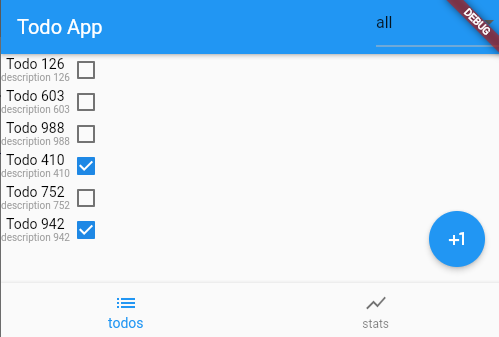
\includegraphics[scale=0.6]{Images/shot_runtime_todoapp.png}
    }
    \quad
    \subfloat[todos tab runtime widget tree.\label{fig:todos_tab_tree}]{
        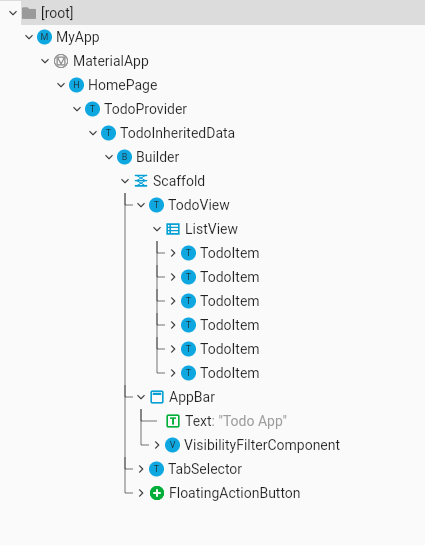
\includegraphics[scale=0.6]{Images/tree_structure_on_HomePage_todos.png}
    }
    \caption{Show the runtime Widget's tree and UI when visualizing todos tab.}
    \label{fig:todos_tab}
\end{figure}


Figure~\ref{fig:todos_tab_UI} shows how the application's UI looks like after few seconds from the start. Figure~\ref{fig:todos_tab_tree} show the widget's tree related with the run. Notice the TodoInheritedData widget as a child of the HomePage widget,it provides the state to the subtree.
\begin{figure}[H]
    \centering
    \subfloat[stats tab runtime UI.\label{fig:stats_tab_UI}]{
        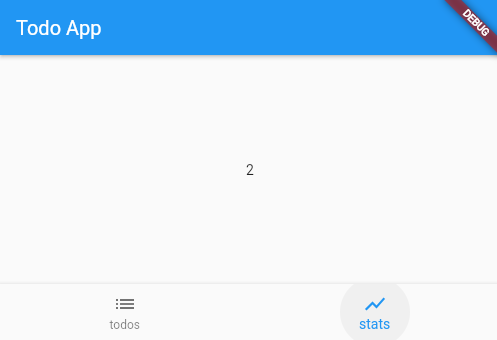
\includegraphics[scale=0.6]{Images/shot_runtime_todoapp_stats.png}
    }
    \quad
    \subfloat[stats tab runtime widget tree.\label{fig:stats_tab_tree}]{
        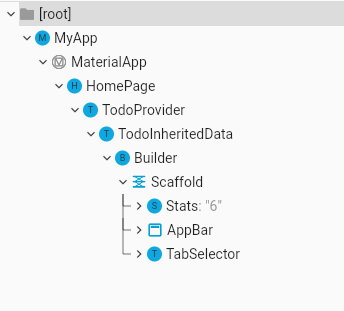
\includegraphics[scale=0.6]{Images/tree_structure_on_HomePage_stats.png}
    }
    \caption{Show the runtime Widget's tree and UI when visualizing stats tab.}
    \label{fig:stats_tab}
\end{figure}

Figure~\ref{fig:stats_tab_UI} shows how the application UI looks like after the user taps on the TabSelector's stats button. Figure~\ref{fig:stats_tab_tree} show the widgets tree related with the run after the button is clicked.\\
\\
Time spent: 2-3 hours\\
Lines of code written/updated: 86\\
Classes/widget created: 2 ( TodoInheritedData class and TodoProvider widget)\\



\paragraph{Features addition} \mbox{} \\
\label{par:feature_addition_inherited_widget}
Here stats the development process where the todo-addition feature and the todo-update feature are implemented.

\subparagraph{Todo addition feature} \mbox{} \\
\label{subpar: todo_addition_feature_inherited_widget}
First thing first, TodoInheritedData widget must provide a function to add todos. A new function is created in the TodoProvider widget and passed to the TodoInheritedData widget. This new function will be called \textit{onAddTodo} and will take two parameters (name and description).
\mbox{}\\


\captionof{listing}{Todo app - InheritedWidget - TodoProvider \textit{onAddTodo} function implementation}
\mbox{}\\
\begin{code}
\label{code:2.31}
\begin{minted}{dart}

void onAddTodo(String name, String desc) {
  Random rand = Random();
  List<int> ids = todos.map((e) => e.id).toList();
  int newId = rand.nextInt(1000) + 2;
  while (ids.contains(newId)) {
    newId = rand.nextInt(1000) + 2;
  }
  Todo newTodo = Todo(
      id: newId,
      name: name,
      description: desc+ " " + newId.toString(),
      completed: false);
  List<Todo> newList = List.from(todos);
  newList.add(newTodo);
  setState(() {
       todos = newList;
  });
}
\end{minted}
\end{code}
\mbox{}\\

After generating a new unique id ,it creates a new Todo object called \textit{newTodo }with the \textit{completed }field set to \textit{false }. Adding the new Todo ,to the TodoProvider’s state \textit{todos }list , requires a bit of workaround. The state of a stateful widget is immutable. Yes, it is a bit counterintuitive but ,as we already said , in functional programming, is generally better to create new instances instead of mutating existing one. Indeed, stateful widget's state can only be changed by the \textit{setState } method. Unfortunately, the method \textit{add} for lists, dart languege provides, is of type void and do not return a new list but add the new value to the existing list's instance. For this reason ,directly calling the \textit{add} method to the TodoProvider’s local lists \textit{todos }will have no effect. That list is immutable and cannot be changed.
TodoProvider’s \textit{todos }list must be completely replaced with a new list containing also the new todo. First ,a new temporary list ,called \textit{newList}, is created and populated with the elements present in the \textit{todos }list. Then, the \textit{newTodo }is added to this new list. At this point, is sufficient to replace the \textit{todos }list with the new one inside the \textit{setState} method.\\
To make the \textit{onAddTodo} function accessible down the tree ,is sufficient to add a new field in the TodoInheritedData widget and pass the function to it, on its creation.
\mbox{}\\

\begin{code}

\captionof{listing}{Todo app - InheritedWidget - onAddTodo function propagation}
mbox{}\\

\label{code:2.32}
\begin{minted}{dart}

class TodoInheritedData extends InheritedWidget {
  {...}
  final void Function(String,String) onAddTodo;

  {...}

@override
Widget build(BuildContext context) {
  return TodoInheritedData(
    todos: todos,
    onChangeFilter: onChangeFilter,
    onAddTodo: onAddTodo,
    onSetCompleted: onSetCompleted,
    filter: filter,
    child: widget.child,
  );
}
\end{minted}
\end{code}
\mbox{}\\

In the AddTodoPage ,a TextButton widget has been already set up and is ready to call the \textit{onAddTodo }function once tapped. However, there is a small inconvenient. The AddTodoPage is accessed by pushing on top of the HomePage another route as shown in figure \ref{fig:add_todo_page_tree_structure}. The AddTodoPage is added as a child of the MaterialApp widget.

\begin{figure}[H]
    \centering
    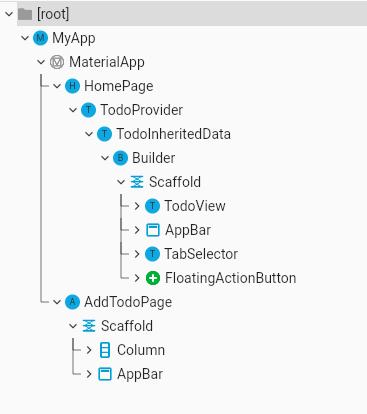
\includegraphics[width=0.6\textwidth]{Images/tree_structure_on_AddTodoPage.png}
    \caption{Show the tree structure after the FloatingActionButton in the HomePage is tapped.}
    \label{fig:add_todo_page_tree_structure}
\end{figure}


The AddTodoPage is not a part of the subtree of the HomePage but is a standalone tree. There is no instance of TodoProvider widget as ancestor of the  Scaffold widget present in the AddTodoPage. Tt is not possible, touogh, to call the \textit{of} method as  we did before. Indeed ,calling the \textit{of} method in a context where a TodoProvider widget is not present will cause the line,
\mbox{}\\

\begin{code}
\label{code:2.33}
\begin{minted}{dart}

assert(result != null, 'No TodoInheritedData found in context');
\end{minted}
\end{code}
\mbox{}\\
inside its implementation, to return \textit{false} and rise a runtime error. The easiest method to proceed is to pass the \textit{onAddTodo} function as a parameter to the AddTodoPage when it is pushed on top of the HomePage. A new parameter, called \textit{addTodoCallback }, is added to the AddTodoPage .
\mbox{}\\


\captionof{listing}{Todo app - InheritedWidget - AddTodoPage's callback function parameter creation}
\mbox{}\\
\begin{code}
\label{code:2.34}
\begin{minted}{dart}

class AddTodoPage extends StatefulWidget {

  final void Function(String,String) addTodoCallback;
    {. . .}
\end{minted}
\end{code}
mbox{}\\
Then, the MaterialApp is notified about the necessity of this new argument at the AddTodoPage creation. It will find the argument inside the context, in a specific variable called \textit{arguments.}
\mbox{}\\


\captionof{listing}{Todo app - InheritedWidget - MaterialApp AddTodoPage route ridefinition}
\mbox{}\\
\begin{code}
\label{code:2.35}
\begin{minted}{dart}

routes: {
{. . .}
  "/addTodo": (context) => AddTodoPage(
      addTodoCallback: ModalRoute.of(context)!.settings.arguments
          as Function(String, String)),
},

\end{minted}
\end{code}
\mbox{}\\

The only part to fill in, in the AddTodoPage, is the \textit{onPressed} field of the TextButton. The callback function in then used, inside it, to add the new todo to the list, then, the AddTodoPage is popped.
\mbox{}\\


\captionof{listing}{Todo app - InheritedWidget - AddTodoPage TextButton onPressed field implementation}
\mbox{}\\ 

\begin{code}
\label{code:2.36}
\begin{minted}{dart}

TextButton(onPressed: () {
  widget.addTodoCallback(textControllerName.text,textControllerDesc.text);
  Navigator.pop(context);
}
\end{minted}
\end{code}
\mbox{}\\

When the AddTodoPage is popped, the new Todo is added and the HomePage is rebuilt.\\
\\

Time spent: 20-30 minutes\\
Lines of code written/updated: 24\\ 
Classes/widget created: 0\\

\subparagraph{Todo updating feature} \mbox{} \\
\label{subpar:todo_updating_feature_inherited_wdiget}
A new function must be implemented ,in the TodoProvider widget ,and passed to the TodoInheritedData widget. This new function will be called \textit{onUpdateTodo } and takes three arguments: the \textit{id} of the todo to be updated, the \textit{newName } that should be set and the \textit{newDesc}.

\mbox{}\\

\begin{code}
\captionof{listing}{Todo app - InheritedWidget - todoProvider's onUpdateTodo function implementation}
\mbox{}\\
\label{code:2.37} 
\begin{minted}{dart}

void onUpdateTodo(int id, String newName,String newDesc) {
  assert(todoExists(id) != null, 'No todo with id : \$id');
  List<Todo> newTodosList = todos.map((element) {
    if (element.id == id) {
      return Todo(
          completed: element.completed,
          description: newDesc,
          name: newName,
          id: element.id);
    } else {
      return element;
    }
  }).toList();
  setState(() {
    todos = newTodosList;
  });
}

\end{minted}
\end{code}
\mbox{}\\


\textit{onUpdateTodo} function first checks if a todo matching the id exists. Then, for the same immutability concept we dealt with in paragraph \ref{par:feature_addition_inherited_widget}, a \textit{newTodosList }is created and populated with the elements inside the \textit{todos }list. Moreover, the todo with the corresponding id is updated with the new name and the new description. Finally, the \textit{todos }list in the TodoProvider stateful widget is replaced with the \textit{newTodosList }using the \textit{setState} method.
This new \textit{onUpdateTodo} method is then made accessible down the tree adding a field to the TodoInheritedData widget and passing the method to id.
\mbox{}\\
\begin{code}

\captionof{listing}{Todo app - InheritedWidget - onUpdateTodo function propagation}
\mbox{}\\

\label{code:2.38}
\begin{minted}{dart}

class TodoInheritedData extends InheritedWidget {
  ...
  final void Function(int, String,String) onUpdateTodo;
  ...


@override
Widget build(BuildContext context) {
  return TodoInheritedData(
    todos: todos,
    onChangeFilter: onChangeFilter,
    onAddTodo: onAddTodo,
    onSetCompleted: onSetCompleted,
    onUpdateTodo: onUpdateTodo,
    filter: filter,
    child: widget.child,
  );
}
\end{minted}
\end{code}
\mbox{}\\
For the same problem faced during the implementation of the todo addition feature ,also in this case, the \textit{onUpdateTodo } function must be passed to the new route (no TodoProvider present in this context) as parameter. A new variable is added to the UpdateTodoPage ,beside the already existent one, called \textit{callback }. This new variable will be of type Function taking two Strings as arguments (the id will be already set up by the calling page).
\begin{code}
\mbox{}\\

\captionof{listing}{Todo app - InheritedWidget - UpdateTodoPage callback variable creation}
\mbox{}\\
\label{code:2.39}
\begin{minted}{dart}

class UpdateTodoPage extends StatefulWidget {
  final Todo todo;
  final void Function(String,String) callback;
 \end{minted}
 \end{code}
 \mbox{}\\

All is ready now to push the UpdateTodoPage on top of the Homepage when the InkWell widget (inside the TodoItem widget) is tapped. However, there is a small extra step to perform before proceeding.  Flutter Navigator ,indeed, allows to pass only a single object ,as argument ,between routes. In this case not only the \textit{onUpdateTodo} function but also a instance of the Todo must be passed to the UpdateTodoPage. For this reason a wrapper class is created with the name \textit{UpdateTodoPageArguments }.
\mbox{}\\
\begin{code}
\captionof{listing}{Todo app - InheritedWidget - onUpdateTodo function propagation}

\label{code:2.40}
\begin{minted}{dart}

class UpdateTodoPageArguments {
  final Todo todo;
  final void Function(String ,String) updateState;

  UpdateTodoPageArguments({required this.todo, required this.updateState});
}
\end{minted}
\end{code}
\mbox{}\\
Inside the InkWell’s \textit{onTap }function ,the corresponding todo and the \textit{onUpdate} function are wrapped into an object of type UpdateTodoPageArguments. This object is then passed to the new route.
\mbox{}\\
\begin{code}
\captionof{listing}{Todo app - InheritedWidget - onUpdateTodo function propagation}
\mbox{}\\
\label{code:2.42}
\begin{minted}{dart}

Navigator.pushNamed(context, "/updateTodo",
    arguments: UpdateTodoPageArguments(
        todo: todo,
        updateState: (String newName,String newDesc) {
          TodoInheritedData.of(context, aspect: 0)
              .onUpdateTodo(todo.id, newName,newDesc);
        }));
\end{minted}
\end{code}
\mbox{}\\
It is necessary to specify to the MaterialApp widget where, the two parameter (necessary for the UpdateTodoPage creation), will be situated. As before , they are putted in a specific variable, inside the context object, called \textit{arguments.}
\mbox{}\\
\begin{code}

\captionof{listing}{Todo app - InheritedWidget - onUpdateTodo function propagation}
\label{code:2.42}
\begin{minted}{dart}

routes: {
  "/": (context) => const HomePage(),
  "/updateTodo": (context) => UpdateTodoPage(
        todo: (ModalRoute.of(context)!.settings.arguments
                as UpdateTodoPageArguments)
            .todo,
        callback: (ModalRoute.of(context)!.settings.arguments
                as UpdateTodoPageArguments)
            .updateState,
      ),
\end{minted}
\end{code}
\mbox{}\\
Now that the \textit{onUpdateTodo } function is set up and  passed to the UpdateTodoPage is  time to call it inside the TextButton \textit{onPressed  }field.
\mbox{}\\
\begin{code}

\captionof{listing}{Todo app - InheritedWidget - onUpdateTodo function propagation}
\label{code:2.43}
\begin{minted}{dart}

TextButton(onPressed: () {

  widget.callback(textControllerName.text,textControllerDesc.text);
  Navigator.pop(context);
},
\end{minted}
\end{code}
\mbox{}\\
At this point, once the user taps the confirm button the page pops, the corresponding todo updates and the HomePage rebuilds.\\
\\
Time spent: 20-30 minutes\\
Lines of code written/updated: 43\\ 
Classes/widget created: 1 for arguments between routes\\


\subparagraph{Render optimizations} \mbox{} \\
\label{subpar:render_optimizations_inherited_widget}
The optimizations performed in this part are explained more in details in paragrph RIFERIMENTO RENDERS OPTIMIZATION. I spent some hours trying to figure out how to make the single TodoItem widget rebuild only, after a non -structural change occurs. When a non-structural change occurs ,may be instresting ,tough, to limitate the tree rebuilding  to widgets affected by the mutation only. For example, when the Checkbox inside a TodoItem is tapped, would be nice to rebuild the TodoItem widget only, and not the entire TodoView widget. After some attempts, I realized that it was just not feasible using InheritedWidgets. InheritedWidget ,indeed ,do not offer this possibility at all. Every widget that access the state ,in the TodoProvider’s subtree , using the \textit{of} method ,is registered as \textit{listener} for state changes. Once a state change occurs ,there are only two possibilities: notify all listeners and rebuild them or notify none. In other words when a state change occurs ,and it must be visualized , the entire TodoProvider’s subtree must be rebuilt unconditionally. Flutter framework ,however, offers a particular widget ,called InheritedModel, to handle this kind of scenario. InheritedModel works as InheritedWidget except for the fact that, when a widget access the state ,(calling the \textit{of} method) it must provide also a new additional parameter, called \textit{aspect}. The \textit{aspect} parameter can be whatever object. For example a String or a Int, but also a more complex data structure. The \textit{aspect} parameter identifies which part (or parts) of the state the widget is registering to. 
With this new additional tool is possible to achive the partial rendering we were looking for. Indeed, with InheritedModel , widgets are rebuilt based on the changed aspect of the state. If a particular widget registered for a particular aspect and a state mutation not affecting that aspect, occurs, the widget is not rebuilt. However, the entire logic defining which aspect of the data changed (when a state transition occurs) must be implemented by the programmer.\\
Proceeding with the optimization process, first thing to do is to substitute the extension to InheritedWidget with the InheritedModel one, in the
TodoInheritedData class.
\mbox{}\\
\begin{code}
\captionof{listing}{Todo app - InheritedModel - extension to InheritedModel }
\mbox{}
\label{code:2.44}
\begin{minted}{dart}

class TodoInheritedData extends InheritedModel<int> {
\end{minted}
\end{code}
\mbox{}\\
I decided to use Ints in order to identify aspects. In particular, widgets that need to rebuild on \textit{filteredTodos} list structural change, will register to the aspect identified with the number 0. Widgets that do never need to rebuild will register to the aspect identified with number 1. Widgets that need to rebuild when a non-structural change occurs affecting the specific Todo with id n  will register to the aspect identified with the number n. (no Todos will have id with value 0 or 1. This is a convention I used to keep things simple. Other ,more complex structure , could be used to avoid this behaviour). 
At this point the method \textit{of}, in the TodoInheritedData widget, should be updated taking into account the aspect parameter. Morevover, the \textit{result} variable should be populated with the static \textit{inheritedFrom  } method belonging to the InheritedModel class, instead of the \textit{dependOnInheritedWidgetOfExactType} method belonging to InheritedWidget class.
\mbox{}\\
\begin{code}
\captionof{listing}{Todo app - InheritedModel -  of method implementation}\mbox{}
\label{code:2.45}
\begin{minted}{dart}

static TodoInheritedData of(BuildContext context, {required int aspect}) {
  final TodoInheritedData? result =
      InheritedModel.inheritFrom<TodoInheritedData>(context, aspect: aspect);
  assert(result != null, 'No TodoInheritedData found in context');
  return result!;
}
\end{minted}
\end{code}
\mbox{}\\
All the lines of code that access the state with the \textit{of} method must now be changed taking into account the new implementation and the new \textit{aspect} argument.
\mbox{}\\

\begin{code}
\label{code:2.47}
\begin{minted}{dart}

TodoInheritedData.of(context, aspect: aspect)
\end{minted}
\end{code}
\mbox{}\\
In particular, the TodoView widget will pass as aspect argument the number 0 declaring that should be notified (and rebuild) only when a structural change occurs.
Instead, TodoItem widgets will pass the corresponding Todo’s \textit{id} in the aspect parameter.
Now that every widget is registered to the desired aspect of the data only, is necessary to “teach”, the TodoInheritedData widget ,how to recognize aspects changes. To do so, InheritedModel provides a method called \textit{updateShouldNotifyDepenedent} that is just like the InheritedWidget’s one, \textit{updateShouldNotify }, but takes as argument also a Set of ints called \textit{dependencies }  (aspects). This method is called once for every widget that registered to state changes. The \textit{dependencies }  variable will contain all aspects the widgets registered to (only one for widget in our case). 
\mbox{}\\
\begin{code}

\captionof{listing}{Todo app - InheritedModel - updateShouldNotifyDepented method implementation}\mbox{}
\label{code:2.46}
\begin{minted}{dart}

@override
bool updateShouldNotifyDependent(
    TodoInheritedData oldWidget, Set<int> dependencies) {
  int currLen = filteredTodos.length;
  int prevLen = oldWidget.filteredTodos.length;
  bool structureRebuildlen = (dependencies.contains(0) && currLen != prevLen);
  if (structureRebuildlen == true) {
    return true;
  } else {
    List<int> currIds = filteredTodos.map((todo) => todo.id).toList();
    List<int> prevIds =
        oldWidget.filteredTodos.map((todo) => todo.id).toList();
    bool sameIds = listEquals(currIds, prevIds);
    bool structureRebuildcomp = (dependencies.contains(0) && !sameIds);
    if (structureRebuildcomp == true) {
      return true;
    } else {
      List<bool> components = [];
      for (var element in filteredTodos) {
        components.add(dependencies.contains(element.id) &&
            !oldWidget.filteredTodos.contains(element));
      }
      bool res = components.fold(false,
          (bool previousValue, bool element) => previousValue || element);
      return res;
    }
  }
}
\end{minted}
\end{code}
\mbox{}\\
This method was tough to code. The method's pseudocode is presented down below. 
\mbox{}\\
\begin{code}
\captionof{listing}{Todo app - InheritedModel - updateShouldNotifyDepented method pseudocode}
\mbox{}
\label{code:2.47}
\begin{minted}{dart}
if( widgetRegisteredForStructuralChange && strucuturalChangeOccured){
        return true;
    }else{
        if( widgetRegisteredForSpecificTodoChange && thatTodoChanged){
            return true;
            }else{
                return false;
    }
}
\end{minted}
\end{code}
\mbox{}\\
At this point , when the TodoItem’s checkbox is tapped the single TodoItem widget is rebuilt. However, no visual changes are shown. The widget rebuilds with the same information as before . This is due to the fact that the \textit{build} method populates its internal widgets based on a local \textit{todo} variable. This variable is populated on the TodoItem widget's creation with a Todo instance provided by the parent widget(TodoView). Indeed, when the TodoView widget instantiates TodoItems  in its ListView, it creates a copy of the corresponding Todo before passing it to the constructor. Even if we changed the information contained in the TodoInheritedData widget, the TodoItem widget do not see any difference.  Its local todo variable , indeed, did not change. The fact that ,before the optimization, TodoItem widgets rebuilt correctly comes from the fact that the transition of the state caused the entire TodoView widget to rebuild. The conseguence was that TodoItems were detroyed and created again using new copies of the data coming from the TodoInheritedData widget. \\
To recap, the performance optimization we were looking for were achieved succesfully but an issue ,regarding the syncronization of the data, arised. The TodoItems widget sees a screenshot of the state different from the one seen by the rest of the application. This is a really bad behavior and is caused by the fact that ,sometimes, during programming , more than one level of information caching is required or used to avoid effort in coding and performance issues. In other words, a local copy of the data is kept and referred to in case of data access in order to optimize the accesses in the main storage that can become quite expensive in large scenarios. A great example of that is the local copy of the database’s data used in many applications. Is more effective to fetch data from the database, save them locally, manipulate this local copy and only in case of real necessity access again the database to store them or retrieve other data. In large applications (but also in small ones like in this cases) more than one level of data caching is used. Particular attention is required to handle those levels to avoid inconsistency in what is visualized and the real data. In this case the \textit{filteredTodos} list actually changed but the UI did not reflect this change. The problem was generate by the fact that a local copy of the real Todo instance was passed to the TodoItem widget. Instead , the "correct" way of handling this scenario is to pass the id of the Todo in the constructor and then use this id to look up for the Todo instance in the centralized state (the TodoInheritedData). This of course will require more computational effort but  will guarantee also a lot more stability and robustness. 
Therefore, TodoItem widget's local variable of type Todo is replaced with a new int variable called \textit{id} that represents the id of the Todo the widget is visualizing. In the \textit{build} method, then, the corresponding Todo is looked up.
\mbox{}\\
\begin{code}
\captionof{listing}{Todo app - InheritedModel - TodoItem widget todo look up}
\mbox{}
\label{code:2.48}
\begin{minted}{dart}

class TodoItem extends StatelessWidget {
  final int id;

  const TodoItem({Key? key, required this.id}) : super(key: key);

  @override
  Widget build(BuildContext context) {
    final Todo todo = TodoInheritedData.of(context, aspect: id)
        .todos
        .where((element) => element.id == id)
        .first;
\end{minted}
\end{code}
\mbox{}\\
At this point the application is working as intentioned and the renders optimization was successfully accomplished. \\
\\
Time spent: 8-10 hours\\
Lines of code written/updated: 49\\ 
Classes/widget created: 0 \\






